\chapter{Titulações por pH e por condutividade}\label{ch:g12:ph-conductivity-titrations}

Uma garrafa de vinagre de vinho traz no rótulo ``acidez de 6 \%'': seis
gramas de ácido etanoico em cada cem gramas de vinagre. Nem o ácido
etanoico nem a sua base conjugada são coloridos, e nenhum permanganato
ajuda aqui. Mas um \omterm{def:g9:acids-bases-ph:ph-paper}{pHmetro} mergulhado no vinagre, ou uma célula que
mede quão bem ele conduz, acompanha a reação com uma base gota a gota, e
a forma da curva mostra exatamente onde fica a \omterm{def:g11:titration:equivalence}{equivalência}. Dez minutos
na bancada, e o rótulo está conferido.

\begin{recall}
Uma \omterm{def:g11:titration:titration}{titulação}, a sua \omterm{def:g11:titration:equivalence}{equivalência} e o \omterm{def:g11:titration:equivalence}{volume de equivalência}
(\cref{ch:g11:titration}); as \omterm{def:g12:ka-and-pka:ka}{constantes de acidez}
(\cref{ch:g12:ka-and-pka}); a relação de Henderson e os indicadores
(\cref{ch:g12:buffers-predominance}); as soluções de \omterm{def:g9:ions:ion}{íons} conduzem
eletricidade (\cref{ch:g9:ions}).
\end{recall}

\begin{omfigure}
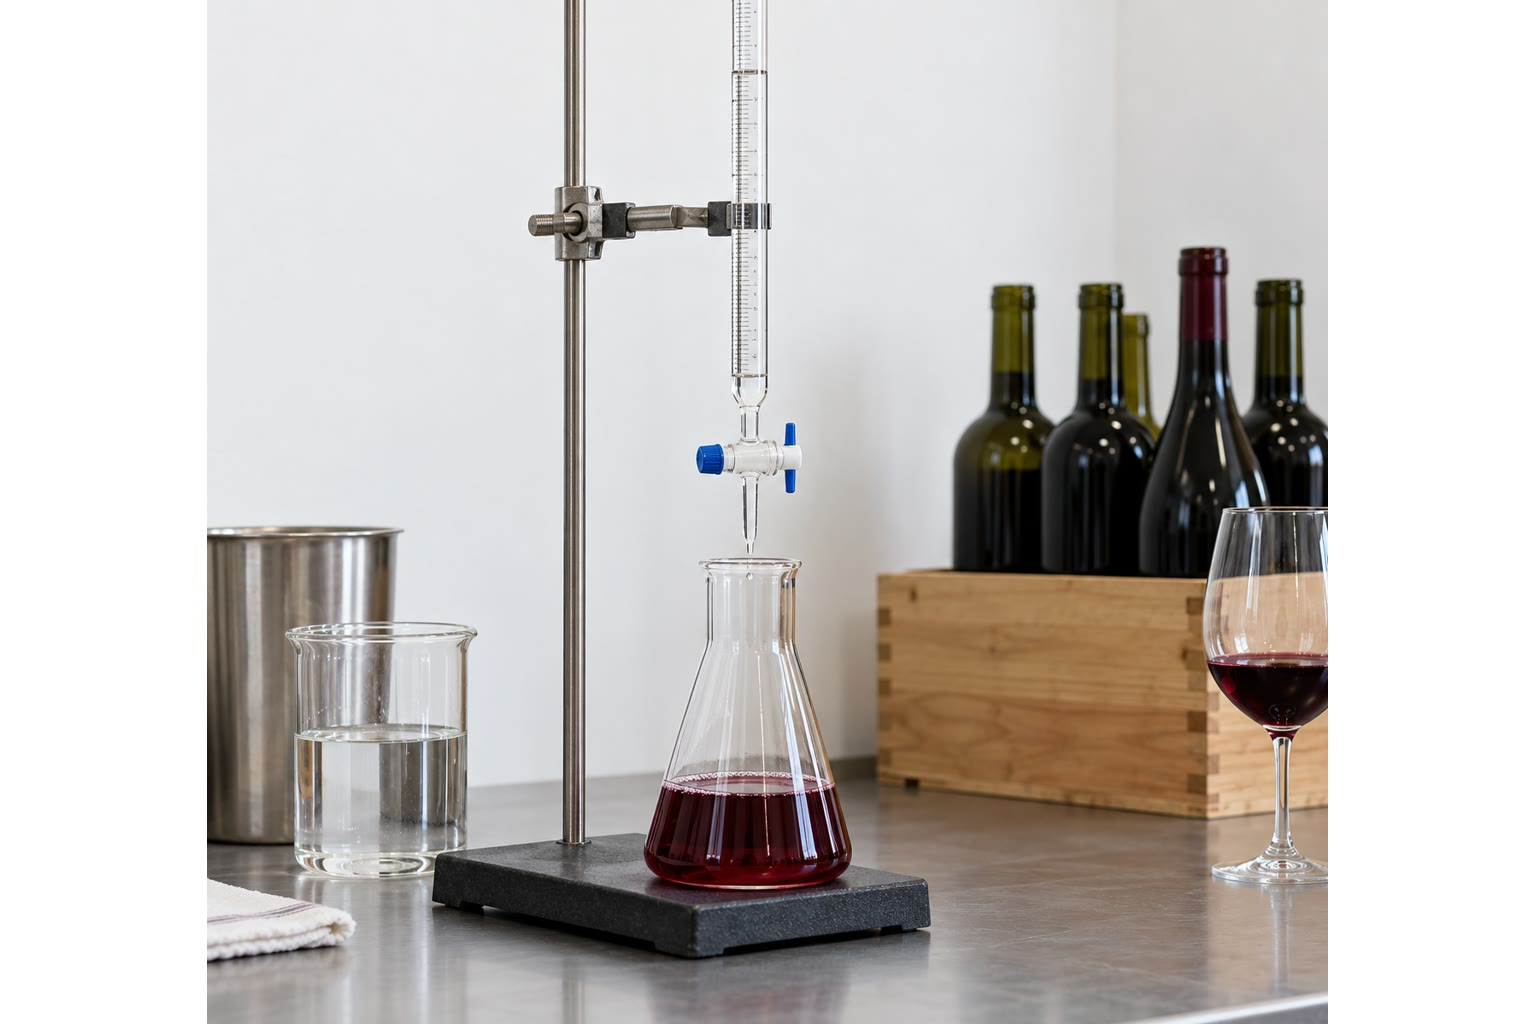
\includegraphics[width=0.45\linewidth]{images/book1/ai/g12-wine-lab.jpg}

{\small A bancada de \omterm{def:g11:titration:titration}{titulação} de um enólogo.}
\end{omfigure}

\section{A titulação potenciométrica}

\begin{definition}[Titulação potenciométrica, semiequivalência]\label{def:g12:ph-conductivity-titrations:ph-metric}
Numa \emph{titulação potenciométrica}\index{titulacao potenciometrica@titulação potenciométrica}, o
\omterm{def:g9:acids-bases-ph:ph}{pH} da \omterm{def:g11:titration:titration}{solução titulada} é medido depois de cada adição de \omterm{def:g11:titration:titration}{titulante}, e
traça-se a curva do \omterm{def:g9:acids-bases-ph:ph}{pH} em função do volume adicionado. A
\emph{semiequivalência}\index{semiequivalencia@semiequivalência} é o ponto em que a
metade do \omterm{def:g11:titration:equivalence}{volume de equivalência} foi adicionada.
\end{definition}

\begin{omfigure}
\begin{tikzpicture}[font=\small, scale=0.65]
  \pic[transform shape] at (0,0) {stand={6.3}{2.0}};
  \pic[transform shape] at (2.0,0.68) {stirrer};
  \pic[transform shape] at (2.0,0.68) {beaker={0.45}{omWater}};
  \pic[transform shape] at (2.0,2.9) {burette={0.8}{omWater}};
  \pic[transform shape] (pr) at (2.6,0.95) {probe};
  \pic[transform shape] (m) at (6.4,3.4) {meter={pH}};
  \draw[black!70, thick] (pr-top) .. controls +(0,1.0) and +(0,-1.2) .. (m-a);
  \draw[omProp, thick, <-] (2.35,7.2) -- (4.3,7.6) node[right, text=black] {bureta: NaOH};
  \draw[omProp, thick, <-] (1.4,1.1) -- (-1.4,1.6) node[left, text=black, align=right] {ácido a titular};
  \draw[omProp, thick, <-] (2.75,2.4) -- (4.3,2.0) node[right, text=black] {eletrodo de pH};
\end{tikzpicture}

{\small Uma \omterm{def:g12:ph-conductivity-titrations:ph-metric}{titulação potenciométrica}: o eletrodo fica mergulhado na
solução agitada, e o aparelho mostra o \omterm{def:g9:acids-bases-ph:ph}{pH} depois de cada adição.}
\end{omfigure}

\begin{inthelab}[Calibrar um pHmetro]
Antes do uso, o eletrodo é enxaguado com água destilada e mergulhado em
duas \omterm{def:g12:buffers-predominance:buffer}{soluções-tampão} de \omterm{def:g9:acids-bases-ph:ph}{pH} conhecido, em geral 7.0 e 4.0 (ou 10.0): o
aparelho é ajustado para indicar esses valores. Entre uma solução e
outra, o eletrodo é enxaguado e seco com leves toques, nunca esfregado;
ele é guardado com a ponta molhada.
\end{inthelab}

\begin{omfigure}
\begin{minipage}{0.49\linewidth}
\begin{tikzpicture}
\begin{axis}[width=\linewidth, height=6cm, xmin=0, xmax=30, ymin=0, ymax=14,
    xlabel={$V_{\text{NaOH}}$ (\si{mL})}, ylabel={pH}, axis lines*=left,
    ymajorgrids, grid style={gray!20}, tick label style={font=\scriptsize},
    label style={font=\small}, title={\small \ce{HCl} por \ce{NaOH}},
    title style={yshift=-4pt}]
  \addplot[very thick, omDef] table[x=V, y=pH] {figdata/out/grade-12-ph-conductivity-titrations-a.dat};
  \addplot[thick, omProp, densely dotted] table[x=V, y expr=\thisrow{dpH}/4]
    {figdata/out/grade-12-ph-conductivity-titrations-a.dat};
  \addplot[dashed, black!60] coordinates {(20,0) (20,7)};
  \node[font=\scriptsize, anchor=north west] at (axis cs:20.3,6.5) {$V_E = 20.0$};
\end{axis}
\end{tikzpicture}
\end{minipage}\hfill
\begin{minipage}{0.49\linewidth}
\begin{tikzpicture}
\begin{axis}[width=\linewidth, height=6cm, xmin=0, xmax=16, ymin=0, ymax=14,
    xlabel={$V_{\text{NaOH}}$ (\si{mL})}, ylabel={pH}, axis lines*=left,
    ymajorgrids, grid style={gray!20}, tick label style={font=\scriptsize},
    label style={font=\small}, title={\small \ce{CH3COOH} por \ce{NaOH}},
    title style={yshift=-4pt}]
  \addplot[very thick, omDef] table[x=V, y=pH] {figdata/out/grade-12-ph-conductivity-titrations-b.dat};
  \addplot[thick, omProp, densely dotted] table[x=V, y expr=\thisrow{dpH}/4]
    {figdata/out/grade-12-ph-conductivity-titrations-b.dat};
  \addplot[dashed, black!60] coordinates {(10.1,0) (10.1,8.7)};
  \addplot[dashed, black!60] coordinates {(0,4.76) (5.05,4.76) (5.05,0)};
  \node[font=\scriptsize, anchor=south west] at (axis cs:0.2,4.8) {$pK_a = 4.76$};
  \node[font=\scriptsize, anchor=north west] at (axis cs:10.4,3.0) {$V_E = 10.1$};
\end{axis}
\end{tikzpicture}
\end{minipage}

{\small Curvas de \omterm{def:g9:acids-bases-ph:ph}{pH} calculadas (em azul) e a sua derivada
$d\mathrm{pH}/dV$ (em laranja, pontilhada, dividida por 4). À esquerda:
\qty{20.0}{mL} de ácido clorídrico a \qty{0.100}{mol/L}; \omterm{def:g11:titration:equivalence}{equivalência} a
\omterm{def:g9:acids-bases-ph:ph}{pH} 7.00. À direita: \qty{10.0}{mL} de vinagre diluído; na
\omterm{def:g12:ph-conductivity-titrations:ph-metric}{semiequivalência}, o \omterm{def:g9:acids-bases-ph:ph}{pH} é igual ao $pK_a$, e a \omterm{def:g11:titration:equivalence}{equivalência} fica num \omterm{def:g9:acids-bases-ph:ph}{pH}
básico.}
\end{omfigure}


\begin{method}[O método da derivada]\label{met:g12:ph-conductivity-titrations:derivative}
Calcule, entre medidas sucessivas, a inclinação
$\Delta\mathrm{pH}/\Delta V$, e trace-a em função de $V$ (uma planilha
ou uma calculadora faz isso). O \omterm{def:g11:titration:equivalence}{volume de equivalência} é onde essa
inclinação é máxima: o pico da curva derivada.
\end{method}

\begin{method}[O método das tangentes]\label{met:g12:ph-conductivity-titrations:tangent}
\begin{enumerate}
  \item Trace duas tangentes paralelas à curva, uma antes e outra depois
        do salto, uma de cada lado dele.
  \item Trace a reta paralela que fica a meio caminho entre elas.
  \item O ponto onde ela corta a curva é o ponto de \omterm{def:g11:titration:equivalence}{equivalência}: leia
        $V_E$ (e o \omterm{def:g9:acids-bases-ph:ph}{pH} na \omterm{def:g11:titration:equivalence}{equivalência}).
\end{enumerate}
\end{method}

\begin{proposition}[Na semiequivalência, $\mathrm{pH} = pK_a$]\label{prop:g12:ph-conductivity-titrations:half}
Na \omterm{def:g11:titration:titration}{titulação} de um \omterm{def:g12:ka-and-pka:strong-acid}{ácido fraco} \ce{HA} por uma \omterm{def:g12:ka-and-pka:strong-acid}{base forte}, na
\omterm{def:g12:ph-conductivity-titrations:ph-metric}{semiequivalência} $\mathrm{pH} = pK_a$.
\end{proposition}

\begin{proof}
A reação \ce{HA + OH- -> A- + H2O} é total. Na \omterm{def:g12:ph-conductivity-titrations:ph-metric}{semiequivalência}, metade
do ácido foi transformada em \ce{A-}: $[\ce{A-}] = [\ce{HA}]$, e a
relação de Henderson dá $\mathrm{pH} = pK_a + \log 1 = pK_a$.
\end{proof}

\begin{remark}[Escolher um indicador a partir da curva]\label{rem:g12:ph-conductivity-titrations:indicator}
% ledger: ind:BBT, ind:phenolphthalein
O indicador deve mudar de cor dentro do salto. Para o ácido clorídrico,
o salto vai de cerca de \omterm{def:g9:acids-bases-ph:ph}{pH} 4 a 10 e muitos indicadores servem, o azul de
bromotimol melhor que todos; para o ácido etanoico, o salto é mais curto
e básico, por volta de 7 a 11: a fenolftaleína (8.0--10.0) serve, o azul
de bromotimol mudaria cedo demais.
\end{remark}

\section{A condutividade e as titulações condutométricas}

\begin{definition}[Condutividade, condutividade iônica molar]\label{def:g12:ph-conductivity-titrations:conductivity}
A \emph{condutividade}\index{condutividade} $\sigma$ de uma solução mede
quão bem ela conduz a eletricidade; ela é lida num condutivímetro em
\si{mS/cm} (ou \si{S/m}). Cada \omterm{def:g9:ions:ion}{íon} $i$ contribui para ela em proporção à
sua concentração, com um coeficiente $\lambda_i$, a sua
\emph{condutividade iônica molar}\index{condutividade ionica molar@condutividade iônica molar}.
\end{definition}

\begin{proposition}[A lei de Kohlrausch]\label{prop:g12:ph-conductivity-titrations:kohlrausch}
% ledger: lam:H+, lam:OH-, lam:Na+, lam:Cl-
Para uma solução diluída, $\sigma = \sum_i \lambda_i [X_i]$. A
\qty{25}{\celsius}, em \si{S.cm^2/mol}: \ce{H3O+} 349.8, \ce{OH-} 198.3,
\ce{Cl-} 76.2, \ce{Na+} 50.3. Os \omterm{def:g12:ka-and-pka:oxonium}{íons oxônio} e hidróxido conduzem muito
melhor que todos os outros \omterm{def:g9:ions:ion}{íons}.
\end{proposition}

\begin{proof}
Admitido (volume do primeiro ano da universidade). Os valores de
\ce{Cl-} e de \ce{Na+} vêm das \omterm{def:g12:ph-conductivity-titrations:conductivity}{condutividades} medidas de soluções de
ácido clorídrico e de cloreto de sódio, das quais se subtrai a do
\ce{H3O+}.
\end{proof}

\begin{definition}[Titulação condutométrica]\label{def:g12:ph-conductivity-titrations:conductimetric}
Numa \emph{titulação condutométrica}\index{titulacao condutometrica@titulação condutométrica}, a
\omterm{def:g12:ph-conductivity-titrations:conductivity}{condutividade} é medida depois de cada adição de \omterm{def:g11:titration:titration}{titulante}. A \omterm{def:g11:titration:titration}{solução
titulada} é diluída num grande volume de água, de modo que o volume
adicionado quase não a mude: os pontos ficam então sobre retas, que
mudam de inclinação na \omterm{def:g11:titration:equivalence}{equivalência}.
\end{definition}

\begin{omfigure}
\begin{minipage}{0.4\linewidth}\centering
\begin{tikzpicture}[font=\small, scale=0.75]
  \pic[transform shape] at (0,0) {beaker={0.6}{omWater}};
  \pic[transform shape] (cc) at (0.2,0.2) {condcell};
  \pic[transform shape] (m) at (2.6,3.4) {meter={mS/cm}};
  \draw[black!70, thick] (cc-top) .. controls +(0,0.8) and +(0,-1) .. (m-a);
  \node[anchor=north, align=center] at (0.6,-0.15) {célula de condutividade\\ na solução};
\end{tikzpicture}
\end{minipage}\hfill
\begin{minipage}{0.56\linewidth}
\begin{tikzpicture}
\begin{axis}[width=\linewidth, height=5.4cm, xmin=0, xmax=20, ymin=0,
    ymax=4.6, xlabel={$V_{\text{NaOH}}$ (\si{mL})}, ylabel={$\sigma$ (\si{mS/cm})},
    axis lines*=left, ymajorgrids, grid style={gray!20},
    tick label style={font=\scriptsize}, label style={font=\small}]
  \addplot[only marks, mark=*, mark size=1.4pt, omDef] table[x=V, y=sigma]
    {figdata/out/grade-12-ph-conductivity-titrations-c.dat};
  \addplot[dashed, black!60] coordinates {(10,0) (10,4.6)};
  \node[font=\scriptsize, anchor=south west] at (axis cs:10.3,0.2) {$V_E = 10.0$};
\end{axis}
\end{tikzpicture}
\end{minipage}

{\small À esquerda: uma célula de \omterm{def:g12:ph-conductivity-titrations:conductivity}{condutividade}. À direita:
\qty{100}{mL} de ácido clorídrico a \qty{0.0100}{mol/L} titulados por
hidróxido de sódio a \qty{0.100}{mol/L} (calculado com a lei de
Kohlrausch). A \omterm{def:g12:ph-conductivity-titrations:conductivity}{condutividade} cai, depois sobe: duas retas que se
encontram na \omterm{def:g11:titration:equivalence}{equivalência}.}
\end{omfigure}

\begin{example}[Ler as duas retas]\label{ex:g12:ph-conductivity-titrations:lines}
Antes da \omterm{def:g11:titration:equivalence}{equivalência}, cada \ce{OH-} adicionado elimina um \ce{H3O+}
($\lambda = 349.8$) e traz um \ce{Na+} ($\lambda = 50.3$): a
\omterm{def:g12:ph-conductivity-titrations:conductivity}{condutividade} cai rapidamente. Depois da \omterm{def:g11:titration:equivalence}{equivalência}, o \ce{Na+} e o
\ce{OH-} ($\lambda = 198.3$) simplesmente se acumulam: ela sobe. As duas
retas se encontram em $V_E = \qty{10.0}{mL}$, logo o ácido estava a
$0.100 \times 10.0 / 100 = \qty{0.0100}{mol/L}$.
\end{example}

\begin{method}[A equivalência numa titulação condutométrica]\label{met:g12:ph-conductivity-titrations:two-lines}
Trace a melhor reta pelos pontos antes da \omterm{def:g11:titration:equivalence}{equivalência} e a melhor reta
pelos pontos depois dela; leia $V_E$ na sua interseção. Os pontos perto
da \omterm{def:g11:titration:equivalence}{equivalência}, onde as retas se curvam, são deixados de lado.
\end{method}

\begin{remark}[Que método usar, e quando]\label{rem:g12:ph-conductivity-titrations:which}
Um indicador colorido é o mais rápido quando existe um adequado. Uma
\omterm{def:g12:ph-conductivity-titrations:ph-metric}{titulação potenciométrica} dá também o $pK_a$ de um \omterm{def:g12:ka-and-pka:strong-acid}{ácido fraco}, e
funciona com soluções coloridas ou turvas. Uma \omterm{def:g12:ph-conductivity-titrations:conductimetric}{titulação condutométrica}
não precisa de nenhum salto de \omterm{def:g9:acids-bases-ph:ph}{pH}: ela funciona para ácidos muito fracos
ou muito diluídos, e para reações de \omterm{def:g9:ions:precipitate}{precipitação}, desde que os \omterm{def:g9:ions:ion}{íons}
mudem.
\end{remark}

\begin{safety}{\ghs[0.82cm]{GHS05}\ghs[0.82cm]{GHS07}}
% ledger: ghs:NaOH
As soluções de hidróxido de sódio queimam a pele e os olhos, até as
diluídas, nos olhos: óculos de proteção o tempo todo, e qualquer
respingo é enxaguado na hora com muita água.
\end{safety}

\section{Exercícios}


\begin{exercise}[$\star$]\label{exo:g12:ph-conductivity-titrations:1}
Leia o \omterm{def:g11:titration:equivalence}{volume de equivalência} na curva do ácido clorídrico titulado por
hidróxido de sódio a \qty{0.100}{mol/L}, e deduza a concentração dos
\qty{20.0}{mL} de ácido.
\end{exercise}

\begin{exercise}[$\star$]\label{exo:g12:ph-conductivity-titrations:2}
Um \omterm{def:g12:ka-and-pka:strong-acid}{ácido fraco} é titulado por hidróxido de sódio; $V_E = \qty{12.0}{mL}$.
Em \qty{6.0}{mL}, o \omterm{def:g9:acids-bases-ph:ph}{pH} é 3.75. Dê o $pK_a$ do ácido. Que ácido da escala
de $pK_a$ ele poderia ser?
\end{exercise}

\begin{exercise}[$\star$]\label{exo:g12:ph-conductivity-titrations:3}
Que indicador você escolheria para a \omterm{def:g11:titration:titration}{titulação} do ácido etanoico por
hidróxido de sódio? Por que não o vermelho de metila?
\end{exercise}

\begin{exercise}[$\star$]\label{exo:g12:ph-conductivity-titrations:4}
Por que um \omterm{def:g9:acids-bases-ph:ph-paper}{pHmetro} deve ser calibrado antes do uso? Com quê?
\end{exercise}

\begin{exercise}[$\star$]\label{exo:g12:ph-conductivity-titrations:5}
Usando as \omterm{def:g12:ph-conductivity-titrations:conductivity}{condutividades iônicas molares}, ordene os \omterm{def:g9:ions:ion}{íons} \ce{H3O+},
\ce{OH-}, \ce{Na+}, \ce{Cl-} do melhor condutor ao pior.
\end{exercise}

\begin{exercise}[$\star\star$]\label{exo:g12:ph-conductivity-titrations:6}
\qty{20.0}{mL} de uma solução de ácido etanoico precisam de
\qty{14.6}{mL} de hidróxido de sódio a \qty{0.050}{mol/L}. Calcule a sua
concentração.
\end{exercise}

\begin{exercise}[$\star\star$]\label{exo:g12:ph-conductivity-titrations:7}
Perto da \omterm{def:g11:titration:equivalence}{equivalência}, as leituras são: \qty{9.6}{mL}, \omterm{def:g9:acids-bases-ph:ph}{pH} 5.7;
\qty{9.8}{mL}, 6.1; \qty{10.0}{mL}, 7.0; \qty{10.2}{mL}, 10.5;
\qty{10.4}{mL}, 11.0. Calcule $\Delta\mathrm{pH}/\Delta V$ entre pontos
sucessivos e localize $V_E$.
\end{exercise}

\begin{exercise}[$\star\star$]\label{exo:g12:ph-conductivity-titrations:8}
Na \omterm{def:g12:ph-conductivity-titrations:conductimetric}{titulação condutométrica} do ácido clorídrico, explique o sinal da
inclinação antes da \omterm{def:g11:titration:equivalence}{equivalência} e depois dela, usando os \omterm{def:g9:ions:ion}{íons}
presentes.
\end{exercise}

\begin{exercise}[$\star\star$]\label{exo:g12:ph-conductivity-titrations:9}
Esboce a curva condutométrica do ácido etanoico titulado por hidróxido
de sódio. Por que a \omterm{def:g12:ph-conductivity-titrations:conductivity}{condutividade} sobe já antes da \omterm{def:g11:titration:equivalence}{equivalência}?
\end{exercise}

\begin{exercise}[$\star\star$]\label{exo:g12:ph-conductivity-titrations:10}
Na curva calculada do vinagre diluído, leia o \omterm{def:g9:acids-bases-ph:ph}{pH} no início, na
\omterm{def:g12:ph-conductivity-titrations:ph-metric}{semiequivalência} e na \omterm{def:g11:titration:equivalence}{equivalência}. Por que o \omterm{def:g9:acids-bases-ph:ph}{pH} inicial é muito mais
alto que o do ácido clorídrico na mesma concentração?
\end{exercise}

\begin{exercise}[$\star\star$]\label{exo:g12:ph-conductivity-titrations:11}
Por que a \omterm{def:g11:titration:titration}{solução titulada} é diluída num grande volume de água antes de
uma \omterm{def:g12:ph-conductivity-titrations:conductimetric}{titulação condutométrica}?
\end{exercise}

\begin{exercise}[$\star\star\star$]\label{exo:g12:ph-conductivity-titrations:12}
Uma solução contém ao mesmo tempo ácido clorídrico e ácido etanoico. Ela
é titulada por hidróxido de sódio enquanto o \omterm{def:g9:acids-bases-ph:ph}{pH} é medido. Explique por
que a curva mostra dois saltos, e o que mede cada \omterm{def:g11:titration:equivalence}{volume de
equivalência}.
\end{exercise}

\begin{exercise}[$\star\star\star$]\label{exo:g12:ph-conductivity-titrations:13}
Calcule a \omterm{def:g12:ph-conductivity-titrations:conductivity}{condutividade} no início da \omterm{def:g12:ph-conductivity-titrations:conductimetric}{titulação condutométrica} do
capítulo (ácido clorídrico a \qty{0.0100}{mol/L}) e na \omterm{def:g11:titration:equivalence}{equivalência}
(\qty{110}{mL} de solução de cloreto de sódio). Compare com a figura.
\end{exercise}

\begin{exercise}[$\star\star\star$]\label{exo:g12:ph-conductivity-titrations:14}
Um \omterm{def:g9:acids-bases-ph:ph-paper}{pHmetro} mal calibrado indica todos os \omterm{def:g9:acids-bases-ph:ph}{pH} 0.2 acima do valor real.
Que erro isso causa no \omterm{def:g11:titration:equivalence}{volume de equivalência} de uma \omterm{def:g12:ph-conductivity-titrations:ph-metric}{titulação
potenciométrica}? E no $pK_a$ lido na \omterm{def:g12:ph-conductivity-titrations:ph-metric}{semiequivalência}?
\end{exercise}

\begin{exercise}[$\star\star\star$]\label{exo:g12:ph-conductivity-titrations:15}
Por que uma \omterm{def:g12:ph-conductivity-titrations:conductimetric}{titulação condutométrica} consegue acompanhar a reação dos
\omterm{def:g9:ions:ion}{íons} prata com os \omterm{def:g9:ions:ion}{íons} cloreto, \ce{Ag+ + Cl- -> AgCl(s)}, e uma
\omterm{def:g12:ph-conductivity-titrations:ph-metric}{titulação potenciométrica} não? Descreva a curva esperada quando se
adiciona nitrato de prata a cloreto de sódio (tome o $\lambda$ do
\ce{NO3-} próximo do valor do \ce{Cl-}).
\end{exercise}

\section{Problema: o vinagre tem mesmo 6\,\%?}

\begin{problem}[{Problema de fim de semana --- um vinagre com ``acidez de
6 \%'' no rótulo contém mesmo seis gramas de ácido etanoico por cem
gramas?}]
\label{pb:g12:ph-conductivity-titrations:1}
% ledger: pka:ethanoic, ind:phenolphthalein, lam:OH-, lam:Na+, aw:C, aw:H, aw:O
Confere-se um vinagre com ``acidez de 6 \%'' no rótulo. Pesam-se
\qty{100.0}{mL} dele: \qty{101}{g}. O vinagre é diluído dez vezes, e
depois \qty{10.0}{mL} da solução diluída são titulados por hidróxido de
sódio a \qty{0.100}{mol/L}, com um \omterm{def:g9:acids-bases-ph:ph-paper}{pHmetro}; a curva calculada do
capítulo (à direita) coincide com as medidas.

\medskip
\noindent\textbf{Parte I --- Preparar a amostra.}
\begin{enumerate}
  \item O que significa ``acidez de 6 \%''?
  \item Se o rótulo estiver certo, que massa de ácido etanoico contêm
        \qty{100.0}{mL} de vinagre? Que \omterm{def:g10:concentration-and-dilution:molar-concentration}{concentração molar} é essa?
  \item Por que o vinagre é diluído antes da \omterm{def:g11:titration:titration}{titulação}?
  \item Que vidraria se usa para diluí-lo dez vezes?
\end{enumerate}

\medskip
\noindent\textbf{Parte II --- A \omterm{def:g12:ph-conductivity-titrations:ph-metric}{titulação potenciométrica}.}
\begin{enumerate}[resume]
  \item Escreva a equação da reação de \omterm{def:g11:titration:titration}{titulação}.
  \item Leia o \omterm{def:g11:titration:equivalence}{volume de equivalência} na curva.
  \item Calcule a concentração do vinagre diluído.
  \item Deduza a do vinagre.
  \item Leia o \omterm{def:g9:acids-bases-ph:ph}{pH} na \omterm{def:g12:ph-conductivity-titrations:ph-metric}{semiequivalência}. O que ele dá?
  \item Por que o \omterm{def:g9:acids-bases-ph:ph}{pH} na \omterm{def:g11:titration:equivalence}{equivalência} fica acima de 7?
  \item Que indicador teria dado o mesmo resultado?
\end{enumerate}

\medskip
\noindent\textbf{Parte III --- Uma verificação condutométrica.}
\begin{enumerate}[resume]
  \item A \omterm{def:g11:titration:titration}{titulação} é repetida com uma célula de \omterm{def:g12:ph-conductivity-titrations:conductivity}{condutividade}, com a
        amostra diluída em \qty{200}{mL} de água. Que \omterm{def:g9:ions:ion}{íons} aparecem na
        solução antes da \omterm{def:g11:titration:equivalence}{equivalência}?
  \item Por que a \omterm{def:g12:ph-conductivity-titrations:conductivity}{condutividade} só sobe devagar antes da \omterm{def:g11:titration:equivalence}{equivalência}?
  \item Por que ela sobe mais depressa depois?
  \item Por que a \omterm{def:g12:ph-conductivity-titrations:conductivity}{condutividade} é muito baixa no início?
  \item Onde as duas retas deveriam se encontrar?
\end{enumerate}

\medskip
\noindent\textbf{Parte IV --- O veredito.}
\begin{enumerate}[resume]
  \item Calcule a \omterm{def:g10:concentration-and-dilution:mass-concentration}{concentração em massa} de ácido etanoico no vinagre.
  \item Calcule a massa de ácido etanoico em \qty{100.0}{mL} de vinagre.
  \item Deduza a massa de ácido etanoico por \qty{100}{g} de vinagre.
  \item Dê a resposta final: qual é a acidez do vinagre?
\end{enumerate}
\end{problem}
